\section{Introduction}  
Let $T$ be a binary tree with subtrees $T_l$ and $T_r$. We say that $T$ is a \textit{binary search tree} (BST) if it is either an empty binary tree or it contains at least one element $x$ as its root such that  

\begin{itemize}  
    \item $T_l$ and $T_r$ are also BSTs.  
    \item $\forall y \in T_l, y < x$ and $\forall z \in T_r, z > x$.  
\end{itemize}  

Although it is well known that, in the worst case, a BST behaves like a linked list (with the height of the tree being $\Theta(n)$), in this report, we focus on \textit{random BSTs} of size $n$.  

By \textit{random BSTs}, we mean the following: Given a universe of keys $U$ with $|U| = n$, we construct the BST by inserting each element of $U$ exactly once, choosing the insertion order uniformly at random.

\section{Analysis of the Average Cost of Insertions}
\subsection{Theoretical Study}
Let us first analyze the expected cost of inserting an element \( u \in U \) into our BST \( T \). For that, we will consider this cost as the cost of searching for \( u \) in our BST, which is valid since we can assume that, if $u$ does not exist in $T$, our search terminates in any empty subtree with identical probability. 

Let $I_n$ be the expected cost of the insertion of a key $x$ in a random BST of size $n$. Let, also, be $I_{n,q}$ be the expected cost of the insertion of a key $x$ in a random BST which root is the $q-\text{th}$ smallest element. Then, the expected cost of $I_n$ is

\begin{align*}
    I_n &= \frac{1}{n}\sum\limits_{q = 1}^{n} I_{n,q} \\
        &= 1 + \frac{1}{n}\sum\limits_{k=1}^{n} (\frac{1}{n} 0 + \frac{k-1}{n} I_{k-1} + \frac{n-k}{n} I_{n-k}) \\
        &= 1 + \frac{1}{n}\sum\limits_{k=0}^{n-1} (\frac{k}{n} I_{k} + \frac{n-k-1}{n} I_{n-k-1}) \\
        &= 1 + \frac{1}{n^2}\sum\limits_{k=0}^{n-1} (k I_{k} + (n-k-1)I_{n-k-1}) \\
        &= 1 + \frac{2}{n^2}\sum\limits_{k=0}^{n-1} k I_{k}
\end{align*}

We can solve this recurrence using the continuous master theorem. The continuous master theorem solves recurrences of the form

\[
F_n = t_n + \sum\limits_{0 \leq j < n} w_{n,j} F_j
\]

with \( t_n = \Theta(n^a (\log n)^b) \). We proceed as follows:

\begin{itemize}
    \item Determine the values of \( a \) and \( b \): Since \( t_n = \Theta(1) \), it is straightforward to see that \( a = b = 0 \).
    \item Provide a shape function for the weights \( w_{n,j} \): We use the following trick to determine the shape function:

    \[
    w(z) = \lim\limits_{n\to\infty} n \cdot w_{n,z\cdot n} = n \cdot \frac{2zn}{n^2} = 2z.
    \]

    \item Determine the value of 

    \[
    \mathcal{H} = 1 - \int\limits_{0}^{1} w(z) z^a dz.
    \]

    Substituting the values, we obtain:

    \[
    \mathcal{H} = 1 - \int\limits_{0}^{1} 2z dz = 1 - (1 - 0) = 0.
    \]

    \item Since \( \mathcal{H} = 0 \), we need to compute 

    \[
    \mathcal{H'} = -(b+1) \int\limits_{0}^{1} w(z) z^a \ln z \, dz.
    \]

    Substituting the known values,

    \[
    \mathcal{H'} = -1 \int\limits_{0}^{1} 2z \ln z \, dz.
    \]

    This integral can be solved using integration by parts. For the purpose of applying the theorem, we skip the detailed calculation, giving the result:

    \[
    \mathcal{H'} = - (x^2 \ln x - \frac{x^2}{2})\Big|_0^1 = \frac{1}{2}.
    \]

\end{itemize}

Since \( \mathcal{H} = 0 \) and \( \mathcal{H'} \neq 0 \), we use the result

\[
F_n = \frac{t_n}{\mathcal{H'}} \ln n + o(t_n \log n).
\]

Substituting the values, we obtain

\[
I_n = 2\ln n + o(\log n).
\]

Thus, the expected cost of an insertion into a random binary search tree is bounded by \( O(\log n) \).

\subsection{Experimental Study}
Once we have theoretical results on the expected cost of an insertion in a random BST, we can provide experimental results to assess how closely they match the theoretical predictions. For this, we will conduct the following experiment:

\begin{enumerate}
    \item We create a random BST of size \( n \) by generating \( n \) random keys in the interval \( [0,1] \).
    \item After constructing the BST, we generate \( q = 2\cdot n \) random numbers in the interval \( [0,1] \).
    \item For each generated value, we perform a \texttt{find} operation in the BST, counting the number of nodes traversed during the operation.
    \item We sum up the total number of nodes traversed across all \( q \) search operations and compute the average.
    \item We repeat all previous steps with 20 different seeds and compute the final average.
    \item We repeat the entire experiment for different values of \( n \).
\end{enumerate}

I conducted the experiment previously explained with values of $n$ ranging from $10,000$ to $200,000$ in increments of $5,000$, using seeds to generate random numbers from $1989$ (in honor of the year of the first publication of the book \textit{Introduction to Algorithms}, which was a great resource for refreshing my knowledge of BSTs and expected cost!) to $2008$. Figure \ref{fig:plotBoundIns} provides a plot of the values obtained from this experiment, as well as the theoretical bound derived using the continuous master theorem. As we can see, the theoretical bound is respected within the experiment. Additionally, Table 1 presents the errors between the theoretical bound and the experimental results.

\begin{figure}
    \centering
    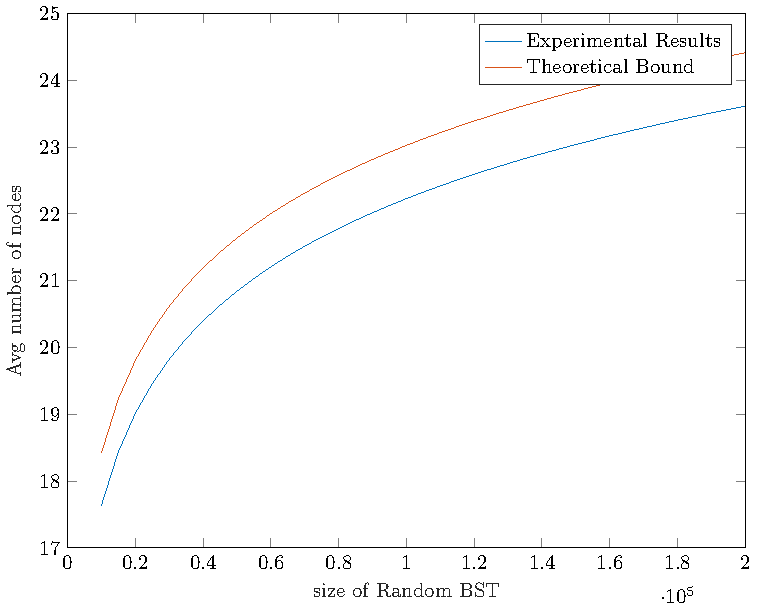
\includegraphics[scale=0.65]{plotInsertion.pdf}
    \caption{Plot}
    \label{fig:plotBoundIns}
\end{figure}

\begin{table}
    \centering
\begin{tabular}{|l|l|l|l|}
\hline 
n & Experimental & Theoretical & Difference \\ 
\hline 
10000 & 17.6373 & 18.4207 & 0.78335 \\ 
15000 & 18.4401 & 19.2316 & 0.79148 \\ 
20000 & 19.0132 & 19.807 & 0.79379 \\ 
25000 & 19.4589 & 20.2533 & 0.79437 \\ 
30000 & 19.8232 & 20.6179 & 0.79466 \\ 
35000 & 20.1327 & 20.9262 & 0.79355 \\ 
40000 & 20.3994 & 21.1933 & 0.79389 \\ 
45000 & 20.6318 & 21.4288 & 0.79707 \\ 
50000 & 20.8435 & 21.6396 & 0.79606 \\ 
55000 & 21.0332 & 21.8302 & 0.79698 \\ 
60000 & 21.2081 & 22.0042 & 0.79606 \\ 
65000 & 21.3695 & 22.1643 & 0.79484 \\ 
70000 & 21.5175 & 22.3125 & 0.79501 \\ 
75000 & 21.6545 & 22.4505 & 0.79602 \\ 
80000 & 21.7826 & 22.5796 & 0.79696 \\ 
85000 & 21.9042 & 22.7008 & 0.79657 \\ 
90000 & 22.0176 & 22.8151 & 0.79753 \\ 
95000 & 22.1266 & 22.9233 & 0.79666 \\ 
100000 & 22.2288 & 23.0259 & 0.7971 \\ 
105000 & 22.3268 & 23.1234 & 0.79667 \\ 
110000 & 22.4196 & 23.2165 & 0.79691 \\ 
115000 & 22.5088 & 23.3054 & 0.79659 \\ 
120000 & 22.5934 & 23.3905 & 0.79713 \\ 
125000 & 22.6754 & 23.4721 & 0.7967 \\ 
130000 & 22.7532 & 23.5506 & 0.79738 \\ 
135000 & 22.8291 & 23.6261 & 0.79692 \\ 
140000 & 22.901 & 23.6988 & 0.7978 \\ 
145000 & 22.9706 & 23.769 & 0.79836 \\ 
150000 & 23.0382 & 23.8368 & 0.79857 \\ 
155000 & 23.1038 & 23.9024 & 0.79857 \\ 
160000 & 23.1678 & 23.9659 & 0.79808 \\ 
165000 & 23.2297 & 24.0274 & 0.79766 \\ 
170000 & 23.2888 & 24.0871 & 0.79832 \\ 
175000 & 23.3468 & 24.1451 & 0.79826 \\ 
180000 & 23.4032 & 24.2014 & 0.79818 \\ 
185000 & 23.4583 & 24.2562 & 0.79793 \\ 
190000 & 23.5112 & 24.3096 & 0.79838 \\ 
195000 & 23.5627 & 24.3615 & 0.79878 \\ 
200000 & 23.6128 & 24.4121 & 0.79932 \\ 
\hline 
\end{tabular}
\caption{xd}
\end{table}

